In Section~\ref{sec: Defining a random walk} we have defined a random walk
model for which we subsequently calculated the fully-coherent mismatch in
Section~\ref{sec: Random walk models part I}. However, this is a special case
in which the random walk for each parameter offset (the difference between the
signal and the template) begins at the origin and then grows with time. It is
the signal which undergoes a random walk, so in this case we have set the
template to exactly match the signal and $t=0$. However, one could imagine choosing
the template in a different way which would reduce the overall mismatch; as such
Eqn.~\eqref{eqn: expectation} may overestimate the mismatch. The proper thing to
do is to minimise the mismatch with respect to the
template parameters~$\lt^{\alpha}$ which are implicitly in the calculation of
Section~\ref{sec: random walk models part I} through
\begin{align}
\Delta \lambda^{\alpha i} = \ls^{\alpha i} - \lt^{\alpha i},
\end{align}
as first defined in Section~\ref{sec: generalising the metric mismatch}.

Ideally, we would like to repeat the calculation leading to Eqn.~\eqref{eqn:
expectation} minimising the mismatch with respect to the template parameters.
However, this calculation has not yet been peformed so a practical alternative
method which we will use here is to begin with the random walk starting at the
origin, as defined in Section~\ref{sec: Defining a random walk}, and then fit and
remove a polynomial of degree $k$. This leaves us with a residual random walk for
which we then compute the mismatch. We will then verify that this captures the
essential features of minimising the mismatch by comparing with numerical
simulations in which the exact mismatch is minimised numerically.

In Appendix~\ref{sec: least squares minimisation of a random walk}, we
introduce the basic tools of least squares fitting and removing a polynomial of
degree $k$ to a generic random walk. In the following sections, we will
calculate the minimised mismatch for random walks in the phase or frequency; we
have not yet calculated the corresponding result for mixtures or random walks
in the spin-down rate. We have a choice in the degree of polynomial to fit and
remove. Since most searches minimise the mismatch with respect to the template
frequency $f_\textrm{t}$ and spin-down rate $\dot{f}_{\textrm{t}}$, this is
equivalent to fitting and removing a $k=2$ polynomial to the phase residual.

\subsection{Random walk in the phase}
\label{sec: minimised rw in phase}
We begin with the simplest case of a random walk in phase, for which we have
\begin{equation}
\Delta\phi_{i} = \s{j=1}{i}\mathcal{N}(0, \sigP).
\end{equation}
Then, as shown in Eqn.~\eqref{eqn: E yiyi} of Appendix~\ref{sec: least squares
minimisation of a random walk}, we have that
\begin{equation}
E[\Delta\phi_{i} \Delta\phi_{j}] = \sigP \min(i, j).
\end{equation}

Then, we define the residual difference between the signal and template
after fitting and removing a $2^{nd}$ order polynomial, $\hat{y}_i^{(2)}$, as
\begin{align}
\Delta^{(2)}\phi_i = \Delta\phi_i - \hat{y}_i^{(2)}.
\label{eqn: D2phi}
\end{align}
Note that the superscript `(2)' indicates the degree of polynomial and by
$\Delta^{(2)}\phi_i$ we mean the residual difference between the signal and
template after fitting and removing the polynomial.

We set the difference between the signal and template in all other parameters
to zero such that the mismatch for a random walk in the residual phase is
therefore
\begin{align}
\mutilde & = g_{0 0 i j} \Delta^{(2)}\phi^{i}\Delta^{(2)}\phi^{j} \\
& = \s{i=1}{\Nsd}g_{00}^{E} \Delta^{(2)}\phi_{i}\Delta^{(2)}\phi_{i}
+ 2 \s{i=1}{\Nsd}\s{j=1}{i-1}g_{00}^{NE}\Delta^{(2)}\phi_{i}\Delta^{(2)}\phi_{j}.
\label{eqn: 4202540871}
\end{align}
To calculate the expectation of the mismatch, we need to evaluate the
expectation of
\begin{align}
\Delta^{(2)}\phi_{i}\Delta^{(2)}\phi_{i} = & \left(\Delta\phi_{i}
- \s{k=1}{\Nsd}\CT_{ik}\Delta\phi_{k}\right)
 \left(\Delta\phi_{j} - \s{l=1}{\Nsd}\CT_{jl}\Delta\phi_{l}\right) \\
= & \Delta\phi_{i}\Delta\phi_{j} -
\left(\s{k=1}{\Nsd}\CT_{ik} \Delta\phi_{j}\Delta\phi_{k}
+ \s{l=1}{\Nsd}\CT_{jl}\Delta\phi_{i}\Delta\phi_{l}\right) \nonumber \\
& +
\s{k=1}{\Nsd}\s{l=1}{\Nsd}\CT_{ik}\CT_{jl} \Delta\phi_{k}\Delta\phi_{l},
\end{align}
where $\CT_{ij}$ is defined in Eqn.~\ref{eqn: C_2} and Eqn.~\ref{eqn:  MCC_2}
of Appendix~\ref{sec: least squares minimisation of a random walk} and we have
replaced $\Delta x$ with the time $\dT$. Then taking the expectation
\begin{align}
\E{\Delta^{(2)}\phi_{i}\Delta^{(2)}\phi_{i}} & =
%E\left[\Delta\phi_{i}\Delta\phi_{j}\right] -
%\left(\s{k=1}{\Nsd}E[\Delta\phi_{j}\Delta\phi_{k}]
%+ \s{l=1}{\Nsd}E[\Delta\phi_{i}\Delta\phi_{l}]\right) +
%\s{k=1}{\Nsd}\s{l=1}{\Nsd}E[\Delta\phi_{k}\Delta\phi_{l}]\\
%& = 
\sigma^{2}_{\phi} \left(\min(i, j) - \left(\s{k=1}{\Nsd}\CT_{ik} \min(j, k)
+ \s{l=1}{\Nsd}\CT_{jl}\min(i, l) \right)\right. \notag \\
& \hspace{13mm} \left. + \s{k=1}{\Nsd}\s{l=1}{\Nsd}\CT_{ik}\CT_{jl}\min(k, l)\right).
\label{eqn: expected mismatch dP0idP0j_k2}
\end{align}
Using symbolic mathematics packages we
calculate an analytic expression which is a function of $\dT, i, j$ and $\Nsd$.
Inserting this into Eqn.~\eqref{eqn: 4202540871} and simplifying we find that
\begin{align}
E[\mutilde]  & = \s{i=1}{\Nsd}g_{00}^{E} E\left[\Delta^{(2)}\phi_{i}\Delta^{(2)}\phi_{i}\right]
+ 2 \s{i=1}{\Nsd}\s{j=1}{i-1}g_{00}^{NE}E\left[\Delta^{(2)}\phi_{i}\Delta^{(2)}\phi_{j}\right]  \\
& = \frac{1}{70}\sigP\left(3N - \frac{27}{\Nsd}\right).
\label{eqn: Expected mismatch RW in phase k2}
\end{align}
This expression can be compared to Eqn.~\eqref{eqn: expectation} ignoring the
effect of the random walk in spin-down rate. Notably, we retain the same
leading order scaling of $\Nsd$, but the overall coefficient is decreased.
Rearranging the expression in the bracket demonstrates the mismatch is negative
or zero for $1 \ge \Nsd \ge 3$: this is a reflection of the minimum number of
points needed in order to perform the quadratic fit. This is shown later in
Sec.~\ref{sec: appendix conclusions} for the simpler case of fitting and
removing a polynomial from a generic random walk.

\subsection{Random walk in the frequency}

For a random walk in the frequency we have an added complexity caused by the
effect the frequency offsets induces in the phase. For the frequency offset we
have
\begin{align}
\Delta f_{i} &= \s{j=1}{i}\mathcal{N}(0, \sigF).
\end{align}
Recalling that we set the reference time at the beginning of each subdomain,
then as in Section~\ref{sec: Defining a random walk}, the induced phase offset is
\begin{align}
\Delta\phi_{i} &=2\pi \s{j=1}{i-1}\Delta f_{j}\dT \\
 & = 2\pi\dT \s{j=1}{i-1}\s{k=1}{j}\mathcal{N}(0, \sigF) \\
& = 2\pi\dT \s{j=1}{i}(i-j)\mathcal{N}(0, \sigF).
\label{eqn: P2F}
\end{align}
Note that we do not include a random walk in the phase here.

Then we calculate the expected values of combinations of the parameter space
offsets
\begin{align}
E[\Delta\f_{i}\Delta\f_{j}] & = \sigF \min(i, j), \label{eqn: E1} \\
E[\Delta\phi_{i}\Delta\f_{j}] & = 2 \pi \dT \sigF \s{k=1}{\min(i, j)}(i-k), \label{eqn: E2}\\
E[\Delta\phi_{i}\Delta\phi_{j}] & =
\left(2\pi\dT\right)^{2}\sigF \s{k=1}{\min(i, j)}(i-k)(j-k).
\label{eqn: E3}
\end{align}

In Eqn.~\eqref{eqn: D2phi}, we defined the residual difference between the signal
and template phase after fitting and removing a scond order polynomial. The
second order polynomial was chosen to model the effect of minimising over the
template frequency and frequency derivative. Let us now define
\begin{align}
\Delta^{(1)}f_i = \Delta f_i - \hat{y}^{(1)},
\label{eqn: D2f}
\end{align}
as the residual difference between the signal and template frequency after
fitting and removing a first order polynomial. In this instance, the first
order polynomial models the effect of minimising over the template
frequency and frequency derivative.

To calculate the mismatch, we expand Eqn.~\eqref{eqn: mismatch} summing over
the residual frequency offset $\Delta^{(1)}f_i$ (defined in Eqn.~\eqref{eqn:
D2f}) and the residual phase offset $\Delta^{(2)}\phi_i$ (given by
subsituting Eqn.~\eqref{eqn: P2F} into Eqn.~\eqref{eqn: D2phi}), this gives
\begin{align}
\begin{split}
E[\mutilde] = &
\s{i=1}{\Nsd}\left(g_{00}^{E}E\left[\Delta^{(2)}\phi_{i}\Delta^{(2)}\phi_{i}\right]
+ 2 g_{01}^{E}E\left[\Delta^{(2)}\phi_{i}\Delta^{(1)}\f_{i}\right]
+  g_{11}^{E} E\left[\Delta^{(2)}\f_{i}\Delta^{(1)}\f_{i}\right] \right) \\
& + 2\s{i=1}{\Nsd}\s{j=1}{i-1}\left(\right.
g_{00}^{NE}E\left[\Delta^{(2)}\phi_{i}\Delta^{(2)}\phi_{j}\right] +
g_{01}^{NE}E\left[\Delta^{(2)}\phi_{j}\Delta^{(2)}\f_{i}\right] +  \\
&\hspace{20mm}\left. g_{10}^{NE}E\left[\Delta^{(2)}\phi_{i}\Delta^{(2)}\f_{j}\right] +
g_{11}^{NE} E\left[\Delta^{(1)}\f_{i}\Delta^{(1)}\f_{j}\right] \right).
\end{split}
\end{align}


We calculate each of these expressions in a similar manner to Eqn.~\eqref{eqn:
expected mismatch dP0idP0j_k2} replacing the relevant expectations with those
given in Eqn.~\eqref{eqn: E1} to Eqn.~\eqref{eqn: E3}. This yields an expected
mismatch given by
\begin{equation}
E[\mutilde] = \frac{\pi^{2} }{630} \sigF \dT^{2}  \left(\Nsd^{3} + 13\Nsd + \frac{82}{\Nsd} \right).
\label{eqn: Expected mismatch RW in frequency k2}
\end{equation}
This can be compared with the frequency noise term alone in Eqn.~\eqref{eqn:
expectation}. We note that the leading order power remains unchanged, but there
is a reduction in the coefficient and a difference in the second highest
power. The reduction in the coefficient is expected since we have minimised
the mismatch; the change in the second highest power is not yet understood.

\subsection{Verification}

We now verify Eqn.~\eqref{eqn: Expected mismatch RW in frequency k2} and
Eqn.~\eqref{eqn: Expected mismatch RW in phase k2} by comparing with Monte
Carlo simulations. The numerical signals undergo a random walk as described in
Section~\ref{sec: Random walk models part I}, however, when searching for the
signals we search over a grid of points in $f_\textrm{t}$ and
$\dot{f}_\textrm{t}$ then select grid point with the minimum mismatch; this
minimises the mismatch over the frequency and spin-down. The results are
plotted in Figure~\ref{fig: verification of minimised RW} and demonstrate good
agreement between the analytic prediction and the mean of the simulated
mismatches.

\begin{figure}[ht]
\centering
\subfloat[Random walk in phase]{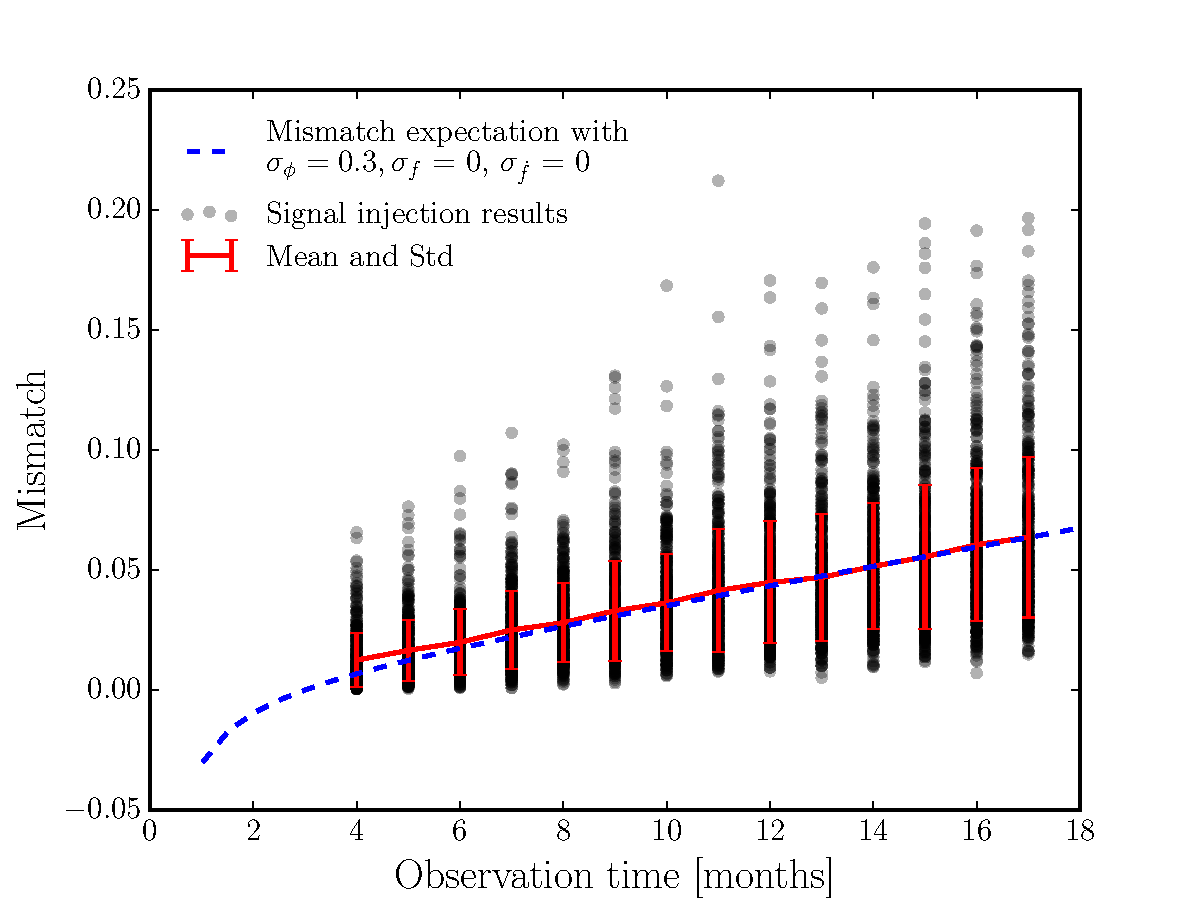
\includegraphics[width=0.5\textwidth]{ExpectationPhase_NarrowBand}}
\subfloat[Random walk in frequency]{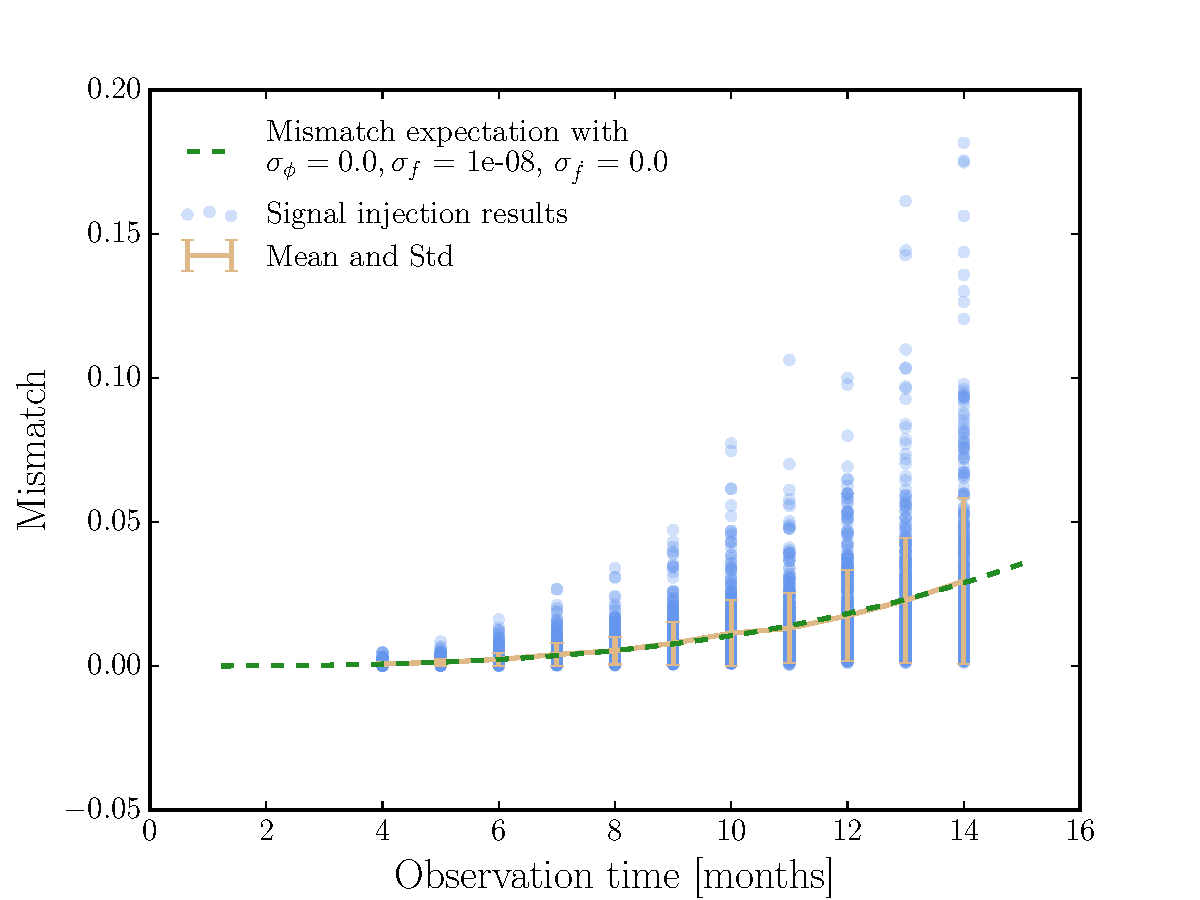
\includegraphics[width=0.5\textwidth]{ExpectationFrequency_NarrowBand}}\\
%\subfloat[Random walk in spin-down]{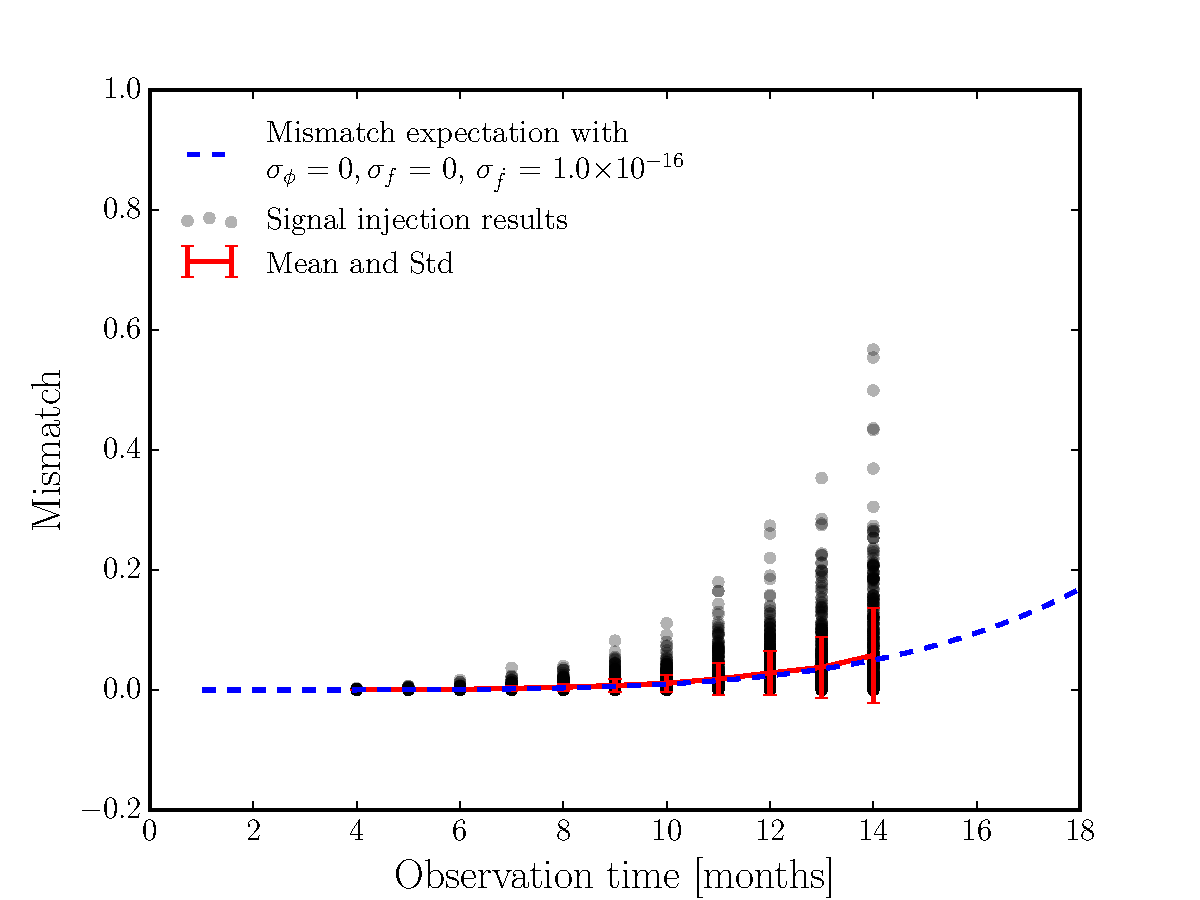
\includegraphics[width=0.5\textwidth]{ExpectationSpindown}}
\caption{A comparison of the Monte Carlo numerical simulated mismatch with the
predictions of Eqn.~\eqref{eqn: Expected mismatch RW in
frequency k2} and Eqn.~\eqref{eqn: Expected mismatch RW in phase k2}; this differs
from Figure~\ref{fig: rw I} in that the numerical mismatch is minimised by selecting
the smallest mismatch from a grid of points in $f_\textrm{t}$ and $\dot{f}_\textrm{t}$.}
\label{fig: verification of minimised RW}
\end{figure}•
\FloatBarrier
